% !TeX encoding = ISO-8859-2

\chapter{Eredm�nyek}
\todoi{meg�rni}



% Please add the following required packages to your document preamble:
% \usepackage{booktabs}
\begin{table}[h]
	\begin{tabular}{@{}|c|c|c|@{}}
		\toprule
		\textbf{Bord�k} & \textbf{Kiszegment�lt bord�k} & \textbf{Helyesen c�mk�zett bord�k} \\ \midrule
		1433            & 1263                          & 727                                \\ \midrule
		100\%           & 88.1\%                        & 50.7\%                             \\ \bottomrule
	\end{tabular}
\centering
\end{table}
\section*{1. eset}
\begin{figure}[h]
	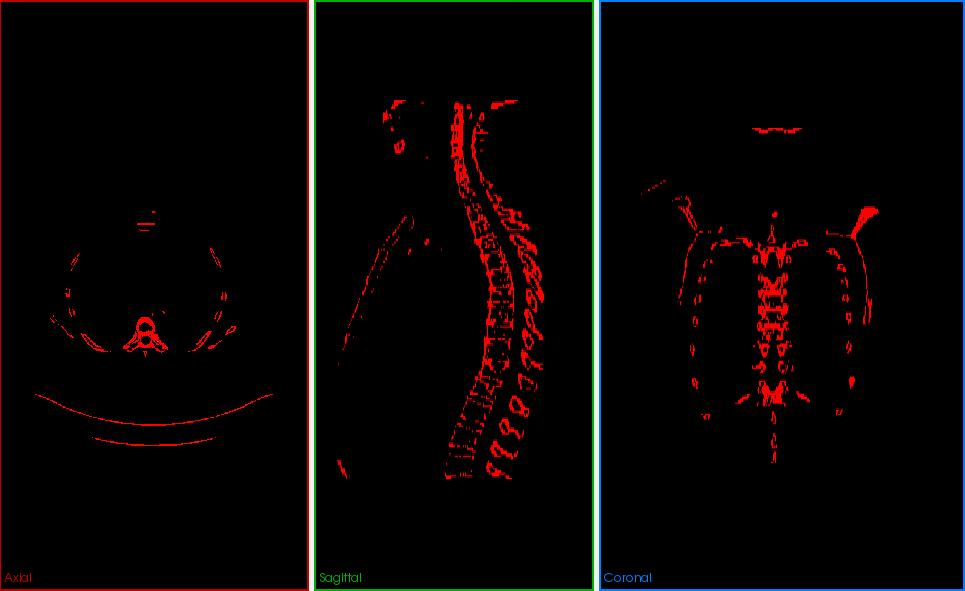
\includegraphics[width=\textwidth]{csont_1_7}
	\centering
	\caption{Csont szegment�l�s} \label{fig:korrig_1_1}
\end{figure}

\begin{figure}[h]
	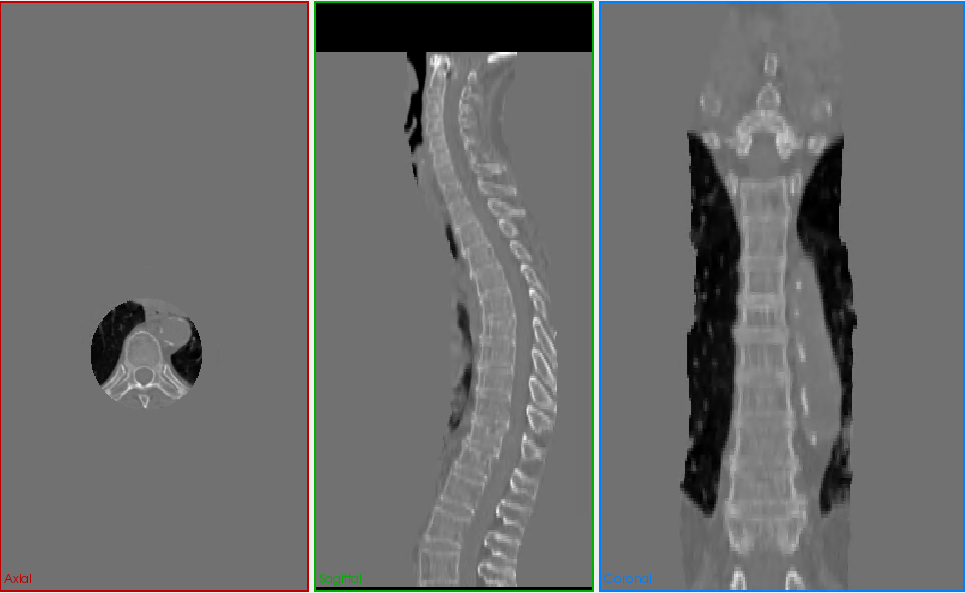
\includegraphics[width=\textwidth]{gerinc_2_7}
	\centering
	\caption{Gerinc kijel�l�s} \label{fig:korrig_1_1}
\end{figure}

\begin{figure}[h]
	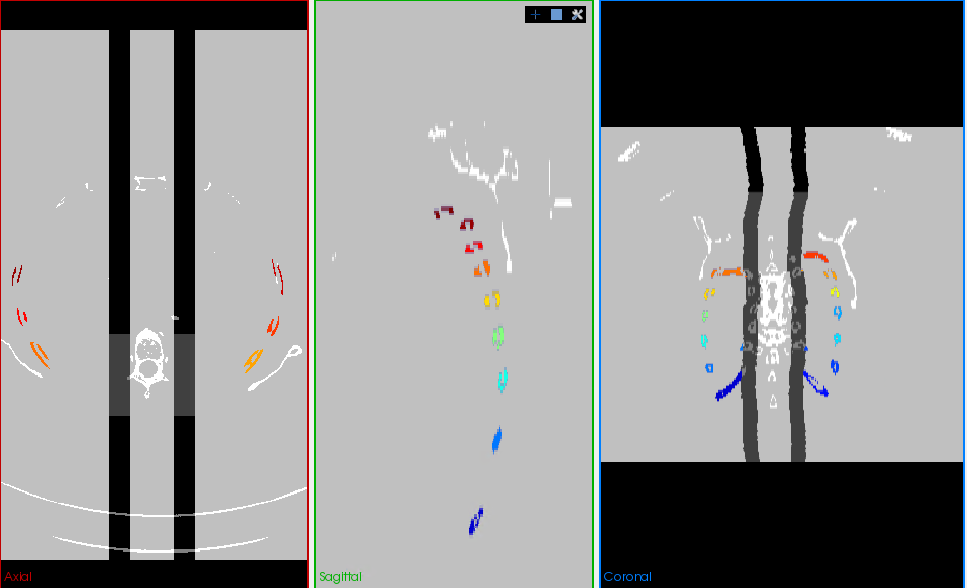
\includegraphics[width=\textwidth]{szeg_3_7}
	\centering
	\caption{R�gi�n�vel�s} \label{fig:korrig_1_1}
\end{figure}
\section*{2. eset}
%-----------------------------------------
\begin{figure}[h]
	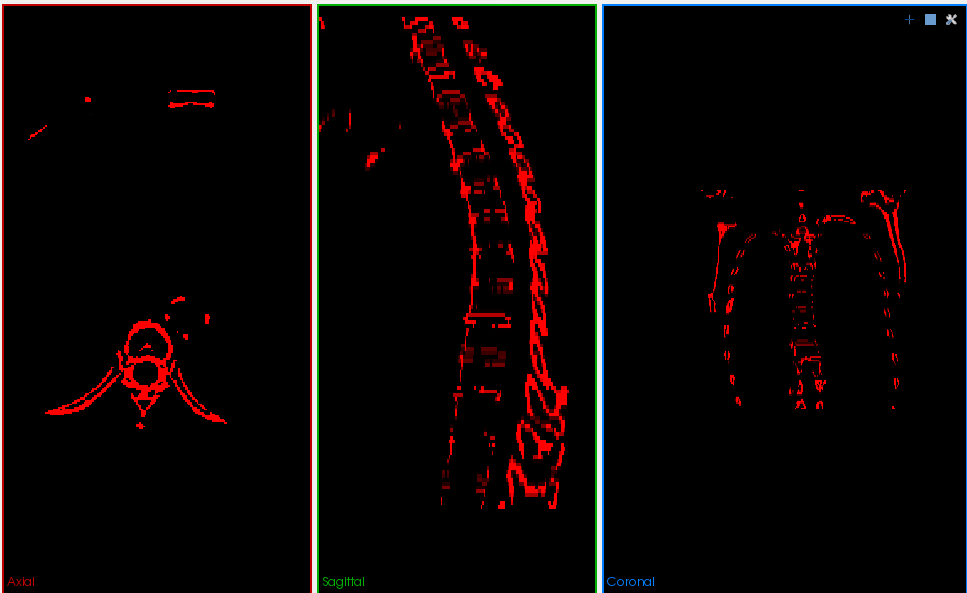
\includegraphics[width=\textwidth]{csont_1_11}
	\centering
	\caption{Csont szegment�l�s} \label{fig:korrig_1_1}
\end{figure}

\begin{figure}[h]
	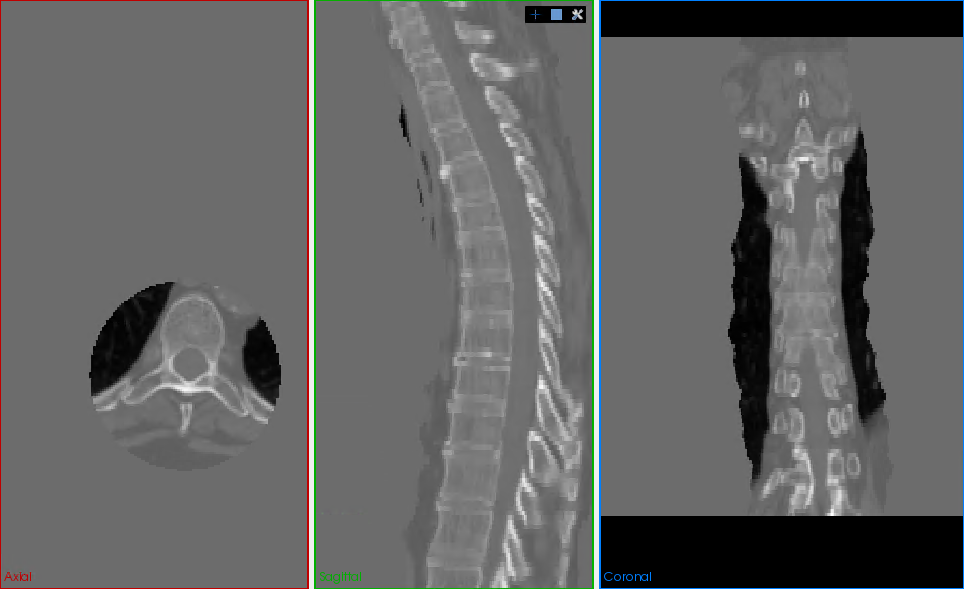
\includegraphics[width=\textwidth]{gerinc_2_11}
	\centering
	\caption{Gerinc kijel�l�s} \label{fig:korrig_1_1}
\end{figure}

\begin{figure}[h]
	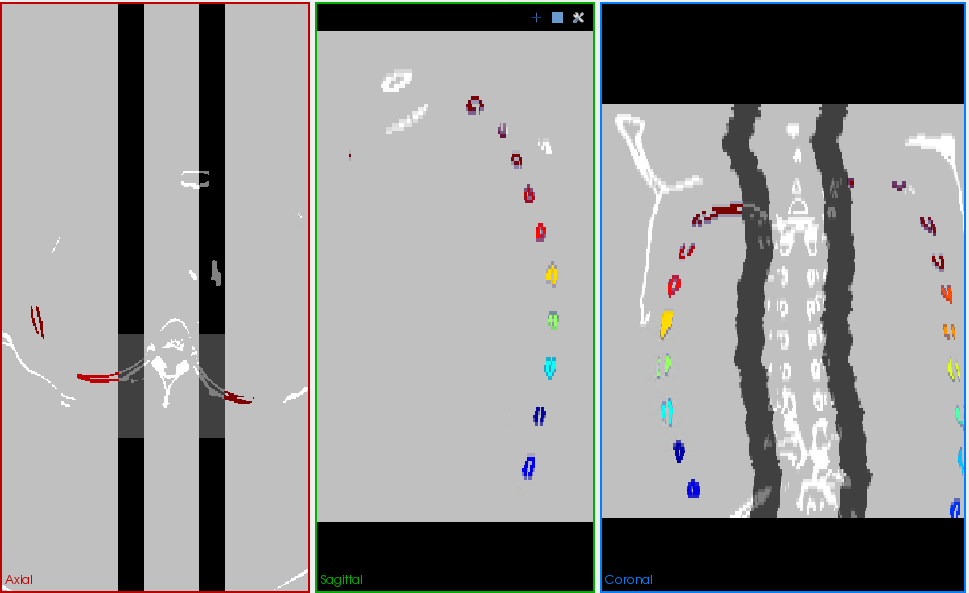
\includegraphics[width=\textwidth]{szeg_3_11}
	\centering
	\caption{R�gi�n�vel�s} \label{fig:korrig_1_1}
\end{figure}
%-----------------------------------------
\section*{3. eset}
\begin{figure}[h]
	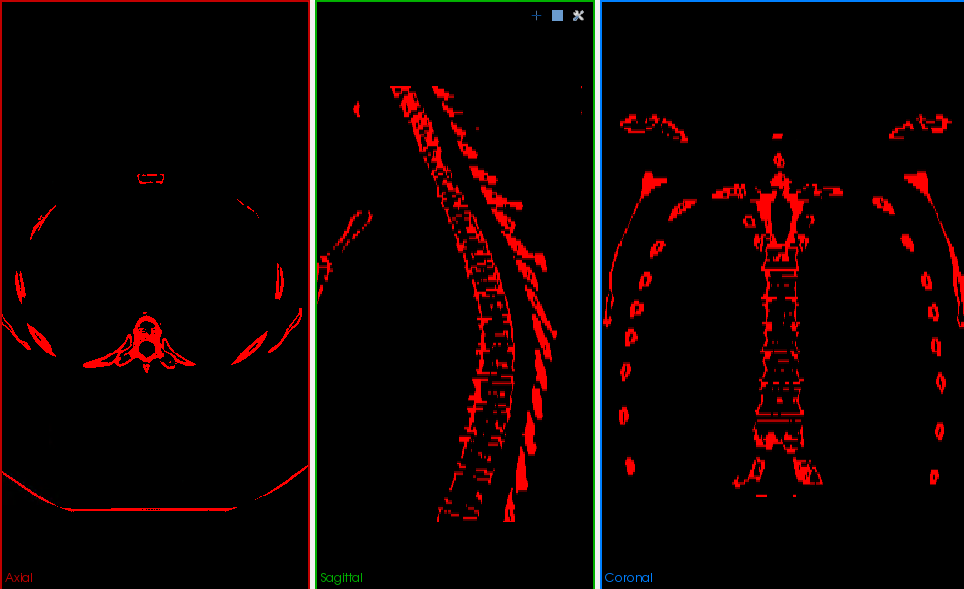
\includegraphics[width=\textwidth]{csont_1_15}
	\centering
	\caption{Csont szegment�l�s} \label{fig:korrig_1_1}
\end{figure}

\begin{figure}[h]
	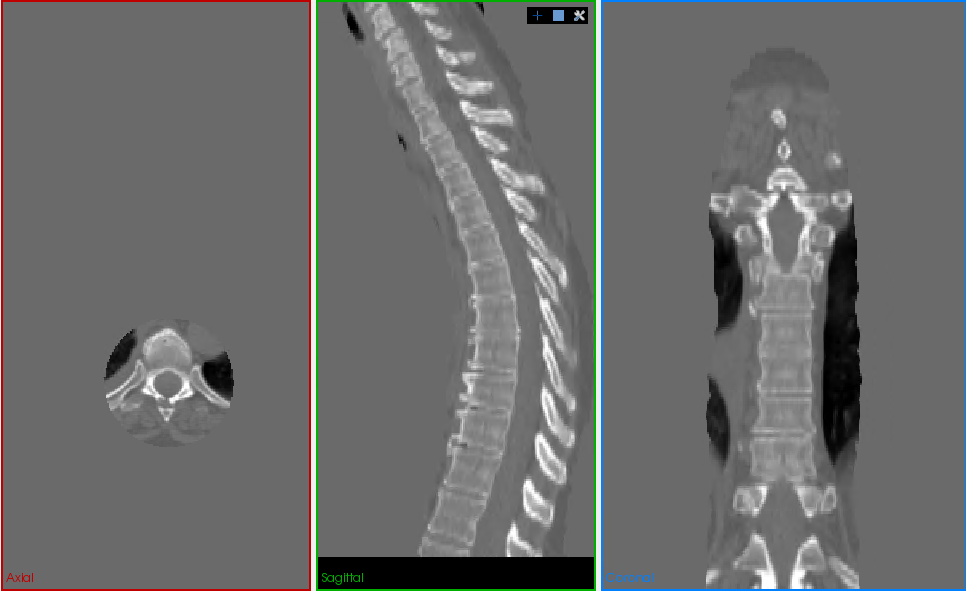
\includegraphics[width=\textwidth]{gerinc_2_15}
	\centering
	\caption{Gerinc kijel�l�s} \label{fig:korrig_1_1}
\end{figure}

\begin{figure}[h]
	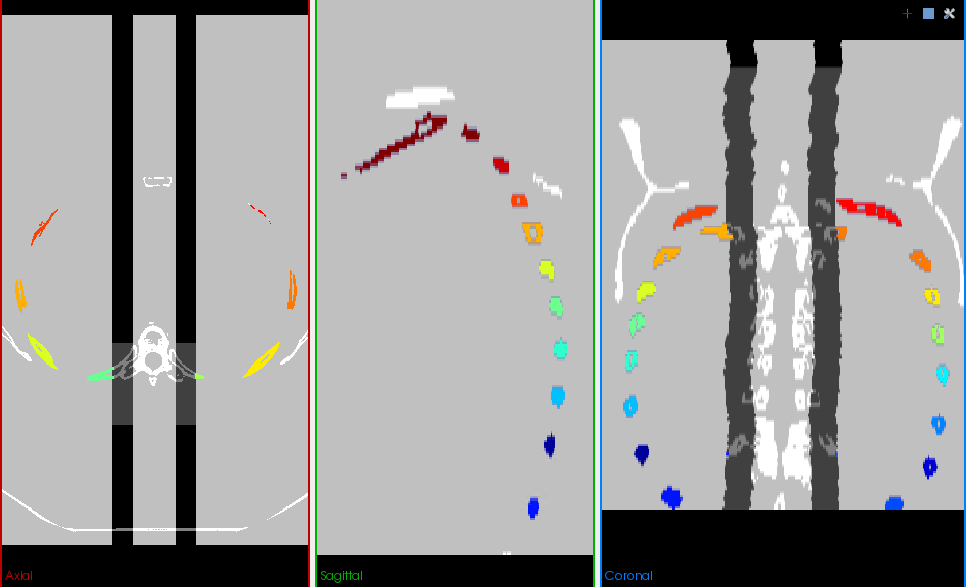
\includegraphics[width=\textwidth]{szeg_3_15}
	\centering
	\caption{R�gi�n�vel�s} \label{fig:korrig_1_1}
\end{figure}
%-----------------------------------------

\begin{comment}
\section{Csont szegment�l�sa}

\section{Gerinc kijel�l�se}

\section{Borda detekt�l�s}

\section{Borda alak� objektumok}

\section{C�mk�zett bord�k}
\end{comment}